% This is "sig-alternate.tex" V2.0 May 2012
% This file should be compiled with V2.5 of "sig-alternate.cls" May 2012
%
% This example file demonstrates the use of the 'sig-alternate.cls'
% V2.5 LaTeX2e document class file. It is for those submitting
% articles to ACM Conference Proceedings WHO DO NOT WISH TO
% STRICTLY ADHERE TO THE SIGS (PUBS-BOARD-ENDORSED) STYLE.
% The 'sig-alternate.cls' file will produce a similar-looking,
% albeit, 'tighter' paper resulting in, invariably, fewer pages.
%
% ----------------------------------------------------------------------------------------------------------------
% This .tex file (and associated .cls V2.5) produces:
%       1) The Permission Statement
%       2) The Conference (location) Info information
%       3) The Copyright Line with ACM data
%       4) NO page numbers
%
% as against the acm_proc_article-sp.cls file which
% DOES NOT produce 1) thru' 3) above.
%
% Using 'sig-alternate.cls' you have control, however, from within
% the source .tex file, over both the CopyrightYear
% (defaulted to 200X) and the ACM Copyright Data
% (defaulted to X-XXXXX-XX-X/XX/XX).
% e.g.
% \CopyrightYear{2007} will cause 2007 to appear in the copyright line.
% \crdata{0-12345-67-8/90/12} will cause 0-12345-67-8/90/12 to appear in the copyright line.
%
% ---------------------------------------------------------------------------------------------------------------
% This .tex source is an example which *does* use
% the .bib file (from which the .bbl file % is produced).
% REMEMBER HOWEVER: After having produced the .bbl file,
% and prior to final submission, you *NEED* to 'insert'
% your .bbl file into your source .tex file so as to provide
% ONE 'self-contained' source file.
%
% ================= IF YOU HAVE QUESTIONS =======================
% Questions regarding the SIGS styles, SIGS policies and
% procedures, Conferences etc. should be sent to
% Adrienne Griscti (griscti@acm.org)
%
% Technical questions _only_ to
% Gerald Murray (murray@hq.acm.org)
% ===============================================================
%
% For tracking purposes - this is V2.0 - May 2012

\documentclass{sig-alternate}
\graphicspath{ {./images/} }

\begin{document}
%
% --- Author Metadata here ---
\conferenceinfo{Knowledge Discovery and Data Mining}{2014, New York, New York USA}
%\CopyrightYear{2007} % Allows default copyright year (20XX) to be over-ridden - IF NEED BE.
%\crdata{0-12345-67-8/90/01}  % Allows default copyright data (0-89791-88-6/97/05) to be over-ridden - IF NEED BE.
% --- End of Author Metadata ---

\title{Data Mining to Improve Traffic Forecasting by Recognizing Anomalies}
%
% You need the command \numberofauthors to handle the 'placement
% and alignment' of the authors beneath the title.
%
% For aesthetic reasons, we recommend 'three authors at a time'
% i.e. three 'name/affiliation blocks' be placed beneath the title.
%
% NOTE: You are NOT restricted in how many 'rows' of
% "name/affiliations" may appear. We just ask that you restrict
% the number of 'columns' to three.
%
% Because of the available 'opening page real-estate'
% we ask you to refrain from putting more than six authors
% (two rows with three columns) beneath the article title.
% More than six makes the first-page appear very cluttered indeed.
%
% Use the \alignauthor commands to handle the names
% and affiliations for an 'aesthetic maximum' of six authors.
% Add names, affiliations, addresses for
% the seventh etc. author(s) as the argument for the
% \additionalauthors command.
% These 'additional authors' will be output/set for you
% without further effort on your part as the last section in
% the body of your article BEFORE References or any Appendices.

\numberofauthors{2} %  in this sample file, there are a *total*
% of EIGHT authors. SIX appear on the 'first-page' (for formatting
% reasons) and the remaining two appear in the \additionalauthors section.
%
\author{
% You can go ahead and credit any number of authors here,
% e.g. one 'row of three' or two rows (consisting of one row of three
% and a second row of one, two or three).
%
% The command \alignauthor (no curly braces needed) should
% precede each author name, affiliation/snail-mail address and
% e-mail address. Additionally, tag each line of
% affiliation/address with \affaddr, and tag the
% e-mail address with \email.
%
% 1st. author
\alignauthor James Howard\\
       \affaddr{Colorado School of Mines}\\
       \affaddr{1500 Illinois St}\\
       \affaddr{Golden, Colorado 80401}\\
       \email{jahoward@mines.edu}
% 2nd. author
\alignauthor William Hoff\\
       \affaddr{Colorado School of Mines}\\
       \affaddr{1500 Illinois St}\\
       \affaddr{Golden, Colrado 80401}\\
       \email{whoff@mines.edu}
}

\maketitle
\begin{abstract}
Accurate traffic forecasting is of great interest for commercial, security, and efficiency applications.  By “traffic”, we mean the movement of vehicles along a road network, the movement of people in a building, or similar data derived from the actions of a group of people.  Traditional forecasting methods use statistical models learned from historical data.  However, the accuracy of these models fail during the presence of anomalies.  In such cases, the forecast can deviate significantly from historical averages.  If anomalies can be observed multiple times, however, then a system can be trained to recognize the anomaly when it is happening and generate a more accurate forecast.  

In this paper, we present a system that automatically discovers anomalies in time series data, and can recognize their occurrence in subsequent data.  We then incorporate these modeled anomalies with common forecasting models to significantly improve short-term forecasting accuracy.  We demonstrate improved short term forecasting accuracy on three datasets:  a publicly available vehicle traffic dataset, and two building occupancy datasets, derived from a sensor network of motion sensors.
\end{abstract}

% A category with the (minimum) three required fields
\category{H.4}{Information Systems Applications}{Miscellaneous}
%A category including the fourth, optional field follows...
\category{D.2.8}{Software Engineering}{Metrics}[complexity measures, performance measures]

\terms{Traffic Forecasting}

\keywords{ACM proceedings}




\section{Introduction}
Human controlled traffic systems are everywhere from the occupancy and motion of people throughout a building to the speed and load of vehicles on a freeway.  With the worlds traffic systems becoming connected, the possibility to dynamically control elements with in that system is at hand.  DISCUSS BRIEFLY THE NEED TO FORECAST OCCUPANCY

What effects can accurate forecasting algorithms have on a system?  According to the United States Department of Transportation, optimal timing of traffic lights on major roadways across the United States could account for approximately a 22\% reduction in emissions along with a 10\% reduction in fuel consumption \cite{DOT2007}.  Similarly, the United Stated Department of Energy \cite{DOE2010} estimates that energy for heating and cooling accounts for approximately 35-45\% of a building's total energy expenditure.  Fully automated building control systems which optimize based on building usage and occupancy can greatly reduce this energy usage.

EMPHASIZE AGAIN THE NEED TO FORECAST ACCURATELY.  PERHAPS DISCUSS THE CURRENT ALGORITHM ACCURACY AND JUSTIFY THE NEED FOR ACCURACY DURING THE TIMES THAT THE SYSTEM IS PERFORMING AT ITS "WORST."

OUTLINE FOR THE REST OF THE PAPER.


\section{Related Work}
TODO TUESDAY MORNING
Work related to traffic forecasting
Work on building occupancy forecasting
Work on Anomaly Detection for time series.
Work on Activity recognition

\section{Notation and Metrics}
\subsection{Notation}
We define a time series dataset used within as  $\{x_{t}^{(m)}\}$.  Each $x_{t}^{m}$ is an aggregate of the readings from sensor $m$ reading at time block $t$.  In total the number of time blocks are represented by $N$.

Forecasts for a given model $k$ from the set of all models $K$ are represented by 
\begin{equation}
y_{t + 1}^{k, m} = f(x_{t}, ..., x_{1}; \theta_{k}).
\end{equation}
\noindent
Thus the forecast of $x_{t + 1}$ is a function of all past data and some trained parameterization $\theta_{k}$ for that model.  For this work we forecast a model for each individual sensor and for convenience often drop the $m$ and $k$ from our forecast notation.  Also, in this work we need to forecast more than one time step into the future.  Future forecasts are performed through iterative one step ahead forecasts.    An example of a forecast two time steps ahead of current time $t$ is given by 
\begin{equation}
y_{t + 2} = f(y_{t + 1}, x_{t}, ..., x_{1}; \theta_{k}).
\end{equation}
\noindent
Such a forecast is simply the forecast for one time step into the future but now with the forecasted value of $y_{t + 1}$ used as the most recent datapoint to forecast $y_{t + 2}$.  Forecasting in this nature allows for forecasts any number of time steps into the future.

Another useful time series used in this work is the residual dataset defined as
\begin{equation}
r_{t,\delta} =  x_{t + \delta} - y_{t + \delta}.
\end{equation}
This set of residuals is the difference between the raw data and a forecasting function operating $\delta$ time steps into the future. 

\subsection{Metrics of Forecasting Accuracy}
We use mean absolute scale error (MASE) \cite{Hyndman2006} and root mean squared error (RMSE) as cost functions to compare with other previously implemented techniques.  These forecasting cost functions are commonly used in forecasting literature and provide a baseline by which to compare our novel forecasting approach to classic forecasting models.  

\bigskip
\noindent \textbf{RMSE} \\
One of the most common error functions used to determine the quality of a set of forecasts.  It measures the average difference between two time series.  In this case, the input series $x$ and the forecast series $y$.
\begin{equation}
RMSE_{\delta} = \sqrt{\frac{\sum_{t = 1}^{N - \delta}{(x_{t + \delta} - y_{t + \delta})^{2}}}{N - \delta}}
\end{equation}

\bigskip
\noindent \textbf{MASE} \\
Mean absolute scaled error was developed to be a generally applicable measurement of forecast accuracy.  The metric is especially useful for datasets with intermittent demand unlike the common closely related measurement of mean absolute percentage error (MAPE).  The reason it works well with intermittent time is that it will not return undefined or infinite values unless all dataset is equal \cite{Hyndman2008}.

\begin{equation}
MASE_{\delta} = \frac{\sum_{t = 1}^{N - \delta}{r_{t, \delta}}}{\frac{N}{N - 1}\sum_{i = 2}^{N}|y_{i} - y_{i - 1}|}
\end{equation}
\subsection{SQEONAN}

\begin{figure}[h]
\centering
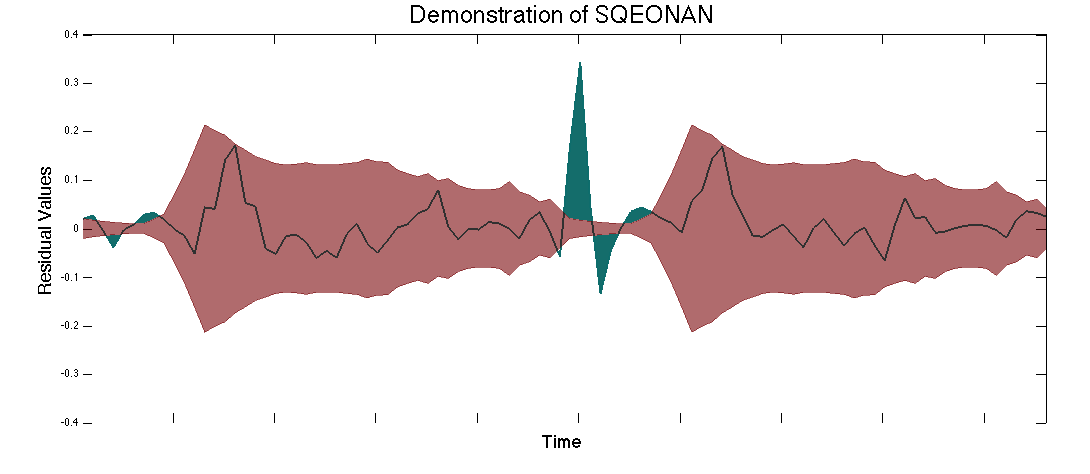
\includegraphics[width = 1.0\linewidth]{demonstration_sqeonan.png}
\caption{A demonstration of the SQEONAN metric.  The sum of the area of all solid teal regions make up the metric.}
\label{fig:sqeonan_demo}
\end{figure}
TODO WE MAY HAVE TO TALK ABOUT $\sigma$ being a vector and not a scalar 

Due to our focus on removing the effects of anomalous events on our forecaster, we can not rely solely on traditional forecasting techniques.  Anomalous events will occur infrequently and thus measures which rely on overall forecasting accuracy will likely not demonstrate much improvement if only the effects of anomalies are removed from our dataset.  We will demonstrate this further at a later time.

To better measure the effect of our approach, we introduce a new measure of forecasting accuracy which we call Sum of Squared Error Outside of Noise Against a Naive Forecaster. SQENAN measures a forecast's accuracy during its worst case scenarios.  This is performed by measuring the sum of squared errors of forecasts outside a prescribed boundary.  We compute this boundary from the forecasting accuracy of a naive forecaster.  For our work, we consider the naive forecaster to be the historical average of the data for a given time.  

The results of this work deal with boundaries set by one and three standard deviations of the residual dataset formed but he historic average (naive) model.  SQEONAN
\begin{equation}
SQEONAN_{\delta, \sigma} = \sum_{t = 1}^{N - \delta}{A(r_{t, \delta}; k\sigma)^{2}} .
\end{equation}
Where $A(r_{\delta}; \sigma)$ is 
\begin{equation}
A(r_{t, \delta}; \sigma_{t}) = \begin{cases}
			r_{t, \delta}    &    \text{If }r_{t, \delta} \ge \sigma_{t} \\
			0                     &    \text{otherwise.}
			\end{cases}
\end{equation}
$\sigma_{t}$ is the standard deviation of the data at that time step for that given day.  For certain comparisons, it is useful to use $k\sigma$ with values of $k > 1$.  

TODO:
Make a note how this is just a sum and thus different length datasets will have different SQEONAN values.  Thus it is difficult to compare performance across datasets.  Instead we should just use this metric to compare the results of various techniques to a given dataset.

An example demonstrating the regions summed by SQEONAN is given by ~\ref{fig:sqeonan_demo}.  In this image, only the area of the teal regions are summed towards the SQEONAN metric.  All other regions are zero.  The large salmon colored region is the area that is one standard deviation for all days at that time for the residual dataset.

\section{Existing Algorithms}
\section{Cluster identification}
\section{Algorithm}

\section{Datasets}
\subsection{Freeway Traffic}
\subsection{Building Traffic}

\section{Results}




\section{Conclusions}

%ACKNOWLEDGMENTS are optional
\section{Acknowledgments}
We acknowledge the support of the National Science Foundation (grant CNS-0931748) as well as Northrop Grumman Corp and Lockheed Martin Corp.

%
% The following two commands are all you need in the
% initial runs of your .tex file to
% produce the bibliography for the citations in your paper.
\bibliographystyle{abbrv}
\bibliography{sigproc}  % sigproc.bib is the name of the Bibliography in this case
% You must have a proper ".bib" file
%  and remember to run:
% latex bibtex latex latex
% to resolve all references
%
% ACM needs 'a single self-contained file'!
%
%APPENDICES are optional
%\balancecolumns
\appendix
\end{document}
